% !Tex TS-program = pdflatex
% !Tex encoding = UTF-8
\documentclass{easyclass}
\usepackage[utf8]{inputenc}
% \usepackage[UTF8]{ctex}
\usepackage{enumitem}
\usepackage{amsmath}
\usepackage{graphics}
\usepackage{hyperref}
\usepackage{color}
\usepackage[
    font={small,sf},
    labelfont=bf,
    format=hang,    
    format=plain,
    margin=0pt,
    width=0.8\textwidth,
]{caption}
\usepackage[list=true]{subcaption}
\begin{document}
\begin{titlepage}
    \university{Wuhan University of Technology}
    \courseid{SLAM}
    \title{Paper Notes}
    \author{Bayes Nie}
    \version{2020 Spring}
    \instructor{Instructors: Dr.~Ins \textsc{Tructor1}\par
    	Dr.~Ins \textsc{Tructor2}, Dr.~Ins \textsc{Tructor3}\par}
    \maketitle
\end{titlepage}

\tableofcontents

\chapter{GraphSLAM  Thrun}
{\large The GraphSLAM Algorithm with Applications to Large-Scale Mapping of Urban Structures}

\section{Preamble}
\textbf{Brief Motivation}: map physical environments with moving sensor platforms to  do: photo-realistic rendering, surveillance, scientific measurement, and robot guidance. 

\textbf{Motivation}: One intuitive way of formulating SLAM is to use a graph whose nodes correspond to the poses of the robot at different points in time and whose edges represent constraints between the poses. The latter are obtained from observations of the environment or from movement actions carried out by the robot. Once such a graph is constructed, the map can be computed by finding the spatial configuration of the nodes that is mostly consistent with the measurements modeled by the edges~\cite{Graph-Based-SLAM-Grisetti}.

\textbf{Related fields}: photogrammetry, computer vision, computer graphics, and robotics.

\textbf{Filter techniques}: a key disadvantage of a filter technique is that data is processed and then discarded. This makes it impossible to revisit all data at the time of map building. 

\textbf{Origin of the SLAM problem}: In robotics, the SLAM problem was introduced through a seminal series of papers by Cheeseman and Smith (1986); Smith and Cheeseman (1986); Smith, Self, and Cheeseman (1990). These papers were the first to describe the well-known EKF SLAM algorithm, often used as a benchmark up to the present day.

\section{GraphSLAM}
\textbf{Basic Intuition}: GraphSLAM extracts from the data a set of soft constraints, represented by a sparse graph. It obtains the map and the robot path by resolving these constraints into a globally consistent estimate. The constraints are generally nonlinear, but in the process of resolving them they are linearized and reduced using variable elimination techniques, arriving at a lower dimensional problems. The resulting least squares problem is solved using standard optimization techniques.

\textbf{Supplementary illustration}: The result of linearization is a sparse information matrix and an information vector. The sparseness of this matrix enables GraphSLAM to apply the variable elimination algorithm, thereby transforming the graph into a much smaller one only defined over robot poses. GraphSLAM also computes a map and certain marginal posteriors over the map; the full map posterior is of course quadratic in the size of the map and hence is usually not recovered.

\textbf{Essence}: graphs of constraints.

\textbf{Two steps}: 
\begin{enumerate}
    \item building a sparse graph of nonlinear constraints.
    \item populating a sparse “information” matrix of linear constraints.
\end{enumerate}

\textbf{Features}: GraphSLAM can handle large number of features, and even incorporate GPS information into the mapping process.

\textbf{Assumption}: 
\begin{enumerate}
    \item static world(map).
    \item feature map.
    \item robot can sense multiple features at each point in time.
    \item robot can only measurement range, hence range measurement.
    \item only determine the mode of the \textit{offline SLAM posterior}. The actual posterior is usually too difficult to express for high-dimensional maps $m$, since it contains dependencies between any pair of features in $m$.
    \item a key assumption in our problem formulation is the assumption of independent Gaussian noise. The Gaussian noise assumption proves convenient in that it leads to a nice set of quadratic equations which can be solved efficiently.
\end{enumerate}

\textbf{Objective}: address \textit{offline SLAM} problem. 
\begin{enumerate}
    \item offline SLAM problem: also called \textit{full SLAM} problem. Seek to calculate a posterior over the \textbf{entire} path $x_{1:t}$ along with the map $m$. 
    \item online SLAM problem: estimate the posterior over the \textbf{momentary} pose along with the map.
\end{enumerate}
The posterior of the full SLAM problem naturally forms a sparse graph. This graph leads to a sum of nonlinear quadratic constraints. Optimizing these constraints yields a maximum likelihood map and a corresponding set of robot poses.

\textbf{correspondence variable}: $j = c_t^i$ means: the $i$-th beam of the measurement at time $t$ detects the feature indexed with $j$.

\subsection{Constructing the Graph}
\textbf{Nodes}: The nodes of this graph are the robot poses $x_{1:t}$ and the features in the map $m = \{m_j\}$.

\textbf{Edges}: Each edge in the graph corresponds to an event: a motion event generates an edge between two robot poses, and a measurement event creates an edge between a pose and a feature in the map.

\textbf{Graph update}: each measurement and each control leads to a local update of $\Omega$ and $\xi$, which corresponds to a local addition of an edge to the graph in GraphSLAM.
\emph{\textbf{An advatange of the information form}: In fact, the rule for incorporating a control or a measurement into $\Omega$ and $\xi$ is a local addition, paying tribute to the important fact that information is an additive quantity.}

\subsection{Sparseness}
\textbf{The graph}: The number of constraints in the graph is linear in the time elapsed, hence the graph is sparse.

\textbf{The matrix}: In the associated information matrix 􏰀, the off-diagonal elements are all zero with two exceptions: between any two consecutive poses $x_{t−1}$ and $x_t$ will be a non-zero value that represents the information link introduced by the control $u_t$. Also non-zero will be any element between a map feature $m_j$ and a pose $x_t$ , if $m_j$ was observed when the robot was at $x_t$ . All elements between pairs of different features remain zero. This reflects the fact that we never receive information pertaining to their relative location--all we receive in SLAM are measurements that constrain the location of a feature relative to a robot pose. Thus, the information matrix is equally sparse; all but a linear number of its elements are zero.

\subsection{Inference}
\textbf{Motivation}: Of course, neither the graph representation nor the information matrix representation gives us what we want: the map and the path.

\textbf{How to obtain}: In GraphSLAM, the map and the path are obtained from the linearized information matrix $\Omega$ and the information vector $\xi$, via the equations $\Sigma = \Omega^{-1} \text{ and } \mu = \Omega^{-1}\xi$

\textbf{Complexity consideration}: 
\begin{enumerate}
    \item \textbf{cycle-free world}: If each feature is seen only locally in time, the graph represented by the constraints is linear. Thus, $\Omega$ can be reordered so that it becomes a band-diagonal matrix, that is, all non-zero values occur near its diagonal. The equation $\mu = \Omega^{-1} \xi$ can then be computed in linear time.
    \item \textbf{cyclic world}: This might be the case because the robot goes back and forth through a corridor, or because the world possesses cycles.Both cases involve features that are observed multiple times. In our constraint graph, this introduces a cyclic dependence: $x_{t_1}$ and $x_{t_2}$ are linked through the sequence of controls $u_{{t_1}+1}$, $u_{{t_1}+2}, \dots, u_{t_2}$ and through the joint observation links between $x_{t_1} \text{ and } m_j$, and $x_{t_2} \text{ and } m_j$, respectively. Such links make our variable reordering trick inapplicable, and recovering the map becomes more complex. 
\end{enumerate}

\subsection{Factorization trick}
\textbf{Motivation}: In fact, since the inverse of $\Omega$ is multiplied with a vector, the result can be computed with optimization techniques such as conjugate gradient, without explicitly computing the full inverse matrix. Since most worlds possess cycles, this is the case of interest. 

\textbf{Intuition}: Simply do marginalization over the feature variables. Think of as propagating information through the information matrix (in fact, it is a generalization of the well-known variable elimination algorithm for matrix inversion). 

\textbf{Result}: An information matrix that only involves poses of robot. However, it is equivalent for the remaining variables, in the sense that the posterior defined by this information matrix is mathematically equivalent to the original posterior before removing $m_j$.
\chapter{Graph-Based SLAM  Grisetti}
{\large A Tutorial on Graph-Based SLAM}

\section{Abstract}
Provide an introductory description to the graph-based SLAM problem. Furthermore, we discuss a state-of-the-art solution that is based on least-squares error minimization and exploits the structure of the SLAM problems during optimization. The goal of this tutorial is to enable the reader to implement the proposed methods from scratch. 

\section{Preamble}
\textbf{SLAM}: Simultaneous Localization and Mapping -- Learning maps under pose uncertainty.

\textbf{Motivation for SLAM}: To efficiently solve many tasks envisioned to be carried out by mobile robots including transportation, search and rescue, or automated vacuum cleaning robots need a map of the environment. The availability of an accurate map allows for the design of systems that can operate in complex environments only based on their on-board sensors and without relying on external reference system like, e.g., GPS.

\textbf{Brief taxonomy for SLAM solutions}:
\begin{enumerate}
    \item \textbf{filtering}: Filtering approaches model the problem as an on-line state estimation where the state of the system consists in the current robot position and the map. The estimate is augmented and refined by incorporating the new measurements as they become available. To highlight their incremental nature, the filtering approaches are usually referred to as on-line SLAM methods.
    \begin{itemize}
        \item Kalman filter and Extended Kalman filter.
        \item Information filter and Extended information filter.
        \item Particle filter.
    \end{itemize}
    \item \textbf{smoothing}: smoothing approaches estimate the full trajectory of the robot from the full set of measurements. These approaches address the so-called full SLAM problem, and they typically rely on least-square error minimization techniques.
\end{enumerate}

\textbf{What can SLAM do}: 
% \begin{figure}[htbp]
%     \centering
%     \begin{minipage}[t]{0.3\textwidth}
%         \centering
%         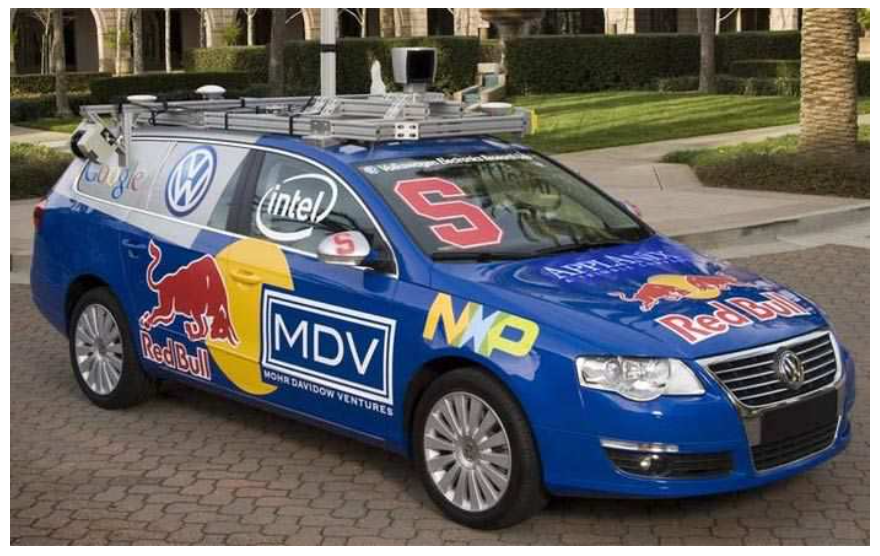
\includegraphics[scale=0.3]{figures/graph_slam/autonomous_parking.png}
%         \caption{Autonomous parking in parking garage}
%     \end{minipage}
%     \begin{minipage}[t]{0.3\textwidth}
%         \centering
%         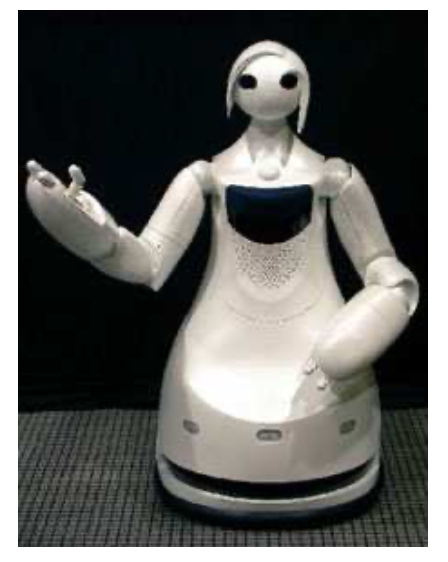
\includegraphics[scale=0.3]{figures/graph_slam/tour_guide.png}
%         \caption{Guiding tours in museum}
%     \end{minipage}
%     \begin{minipage}[t]{0.3\textwidth}
%         \centering
%         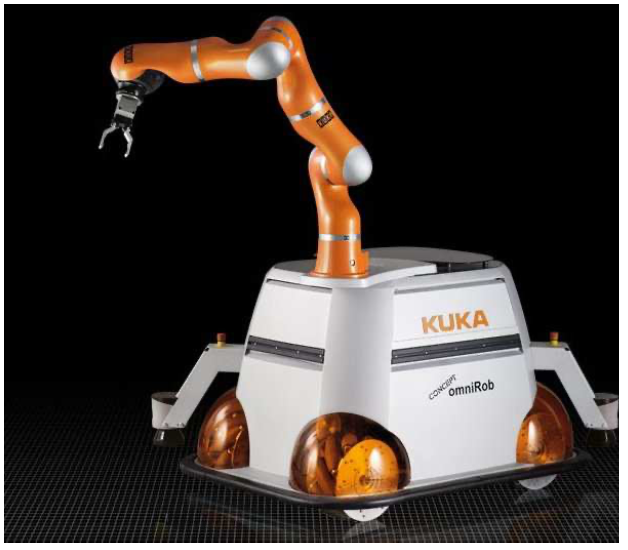
\includegraphics[scale=0.3]{figures/graph_slam/flexible_induestrial_manipulator.png}
%         \caption{Flexibly navigating and operating in changing industrial environment}
%     \end{minipage}
%     % \caption{}
%     \label{fig:what_can_slam_do}
% \end{figure}
\begin{figure}[htbp] 
    \centering
    \subcaptionbox{Autonomous parking in parking garage}{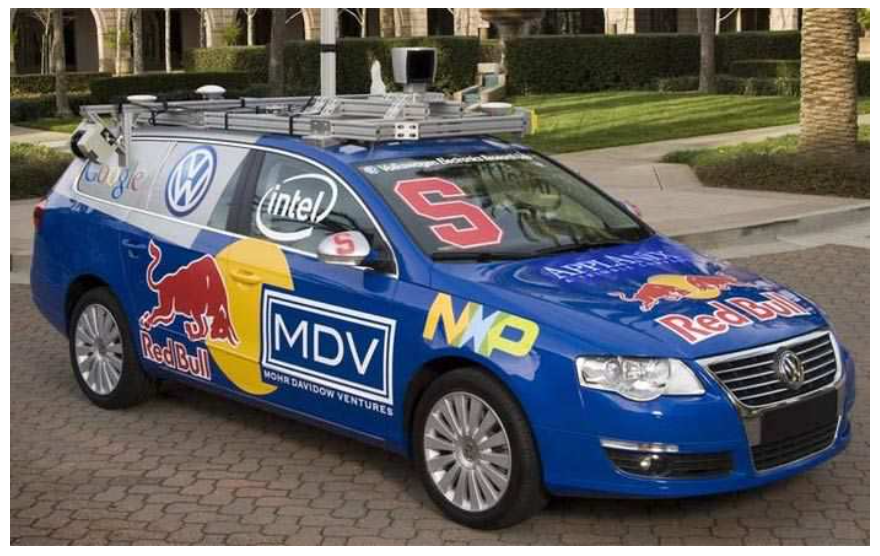
\includegraphics[width=0.3\textwidth]{figures/graph_slam/autonomous_parking.png}}
    \hfill
    \subcaptionbox{Guiding tours in museum}{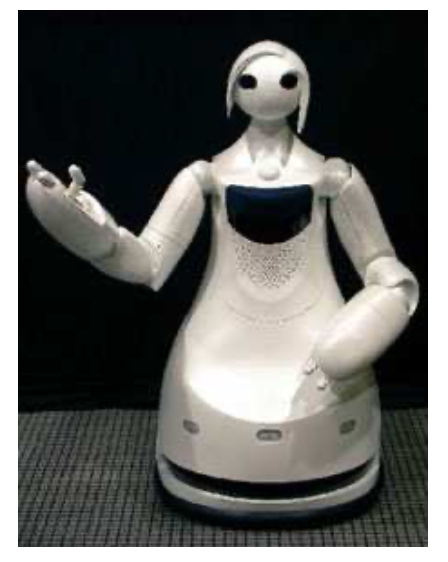
\includegraphics[width=0.3\textwidth]{figures/graph_slam/tour_guide.png}}
    \hfill
    \subcaptionbox{Flexibly navigating and operating in changing industrial environment}{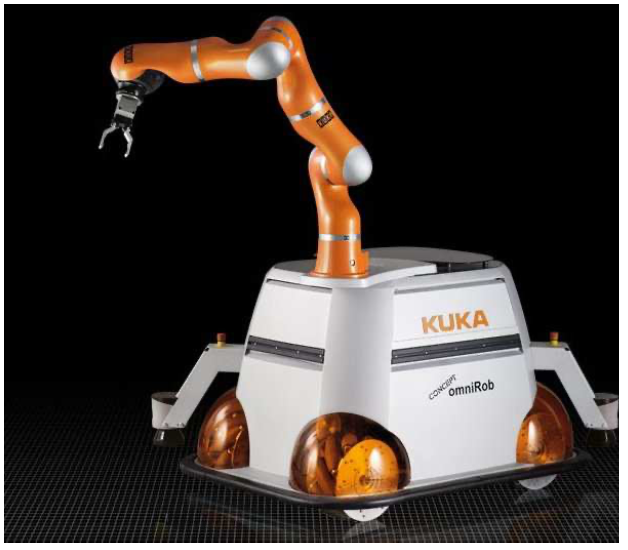
\includegraphics[width=0.3\textwidth]{figures/graph_slam/flexible_induestrial_manipulator.png}}
    \caption{What SLAM can do}
    \label{fig:what_slam_can_do}
\end{figure}

\textbf{Grisetti's elaboration for Graph-Based SLAM}: Solving a graph-based SLAM problem involves to construct a graph whose nodes represent robot poses or landmarks and in which an edge between two nodes encodes a sensor measurement that constrains the connected poses. Obviously, such constraints can be contradictory since observations are always affected by noise. Once such a graph is constructed, the crucial problem is to find a configuration of the nodes that is maximally consistent with the measurements. This involves solving a large error minimization problem. 

\textbf{Grisetti's elaboration for evolution of Graph-Based SLAM}: The graph-based formulation of the SLAM problem has been proposed by Lu and Milios in 1997. However, it took several years to make this formulation popular due to the comparably high complexity of solving the error minimization problem using standard techniques. Recent insights into the structure of the SLAM problem and advancements in the fields of sparse linear algebra resulted in efficient approaches to the optimization problem at hand. Consequently, graph-based SLAM methods have undergone a renaissance and currently belong to the state-of-the-art techniques with respect to speed and accuracy.

\section{Probabilistic formulation of full SLAM}
\textbf{Why probabilistic}: Due to the inherent noise in the sensor measurements. 

\textbf{Full SLAM problem}: 
\begin{equation}
    p(x_{1:t}, m | x_0, u_{1:t}, z_{1:t})
    \label{equ:full_slam_prob}
\end{equation}

\textbf{A bif of elaboration}: 
\begin{enumerate}
    \item The initial position $x_0$ defines the position of the map and can be chosen arbitrarily. Therefore, $x_0$ is always omitted in some SLAM formulations.
    \item The poses and the odometry are usually represented as 2D or 3D transformations in $SE(2)$ or in $SE(3)$.
    \item The map can be represented in different ways ({\color{red} \emph{Need more specific taxonomy of representations of map in SLAM}}):

    \begin{figure}[htbp]
        \centering
        \subcaptionbox{Multilevel surface maps}{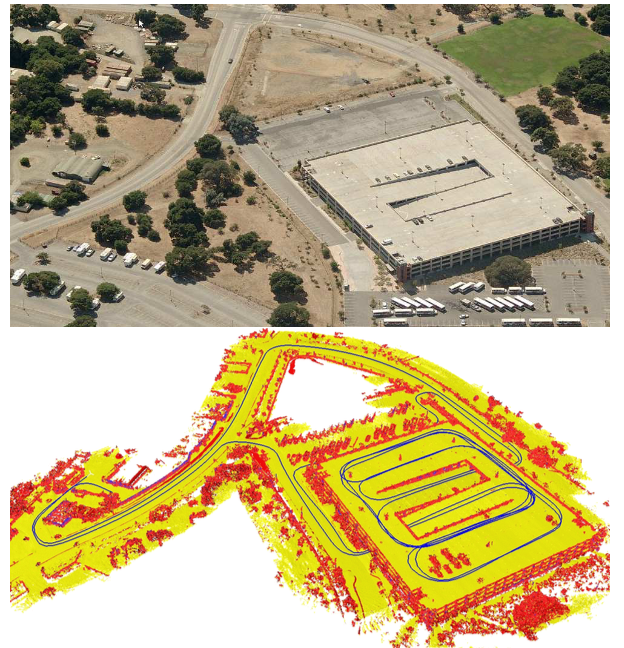
\includegraphics[width=0.3\textwidth]{figures/graph_slam/multilevel_surface_map.png}}
        \hfill
        \subcaptionbox{Point clouds map}{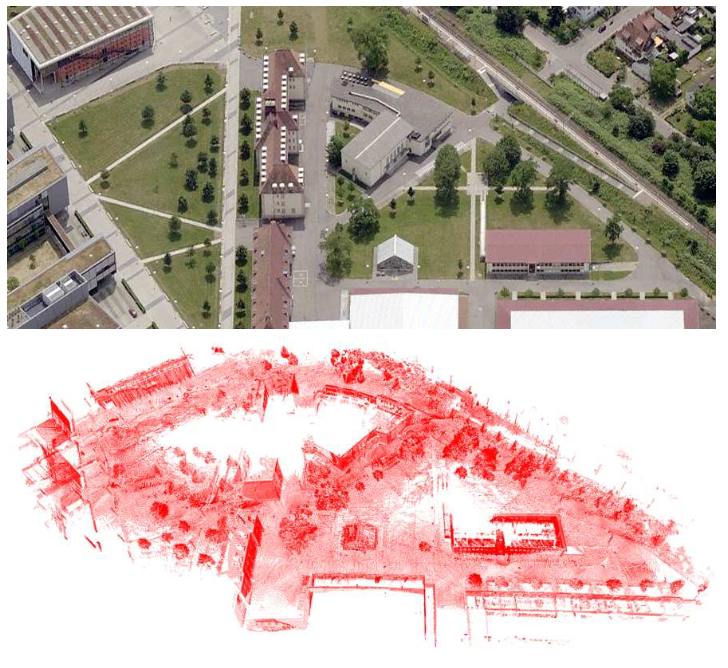
\includegraphics[width=0.3\textwidth]{figures/graph_slam/point_clouds_map.png}}
        \hfill
        \subcaptionbox{Occupancy grid map}{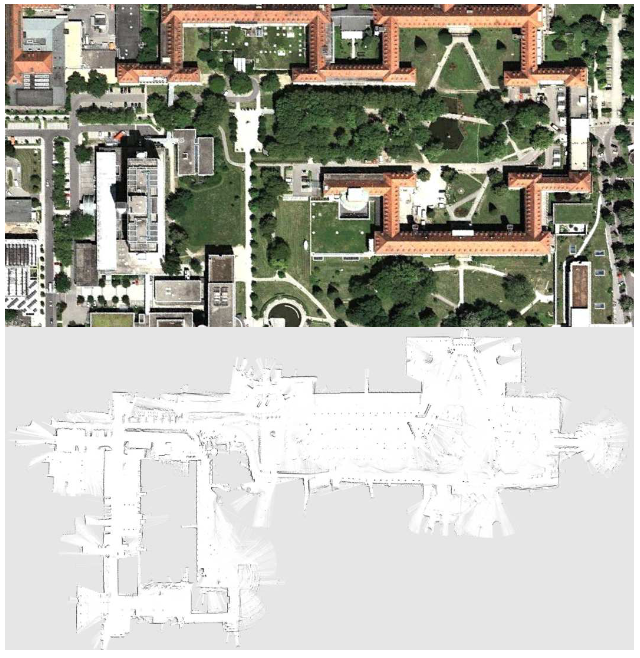
\includegraphics[width=0.3\textwidth]{figures/graph_slam/occupancy_grid_map.png}}
        \caption{Dense representations of the map}
        \label{fig:map_dense_representations}
    \end{figure}
    \begin{itemize}
        \item Maps can be parametrized as a set of spatially located landmarks, by dense representations:
        \begin{itemize}
            \item occupancy grids.
            \item point clouds.
            \item multilevel surface maps.
        \end{itemize}
        \item Or by raw sensor measurements.
    \end{itemize}
    \item The choice of a particular map representation depends on the sensors used, on the characteristics of the environment, and on the estimation algorithm. 
    \item Landmark maps are often preferred in environments where locally distinguishable features can be identified and especially when cameras are used. In contrast, dense representations are usually used in conjunction with range sensors. Independently of the type of the representation, the map is defined by the measurements and the locations where these measurements have been acquired.
\end{enumerate}

\section{Graphical formulation of full SLAM}
\textbf{Motivation for using graphical model}: Estimating the posterior given in \ref{equ:full_slam_prob} involves operating in high dimensional state spaces. This would not be tractable if the SLAM problem would not have a well defined structure. 

\begin{figure}[htbp]
    \centering
    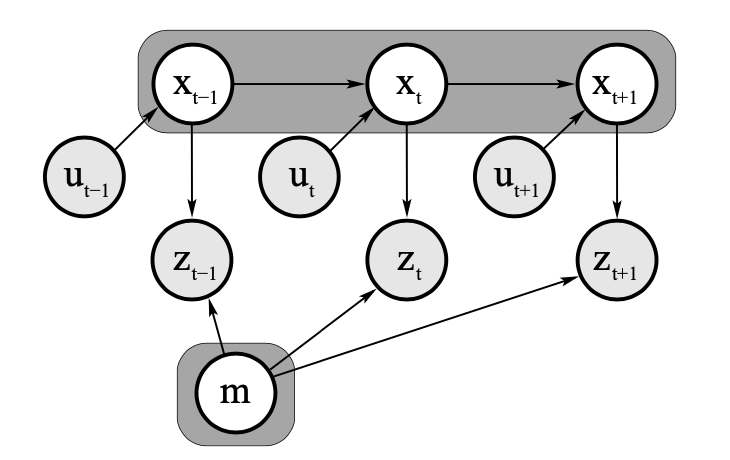
\includegraphics[width=0.5\textwidth]{figures/graph_slam/full_slam_graphical_model.png}
    \caption{Dynamic Bayesian Network of the full SLAM process}
    \label{fig:full_slam_dbn}
\end{figure}


\textbf{Dynamic Bayesian Network}: A convenient way to describe this structure is via the Dynamic Bayesian Network (DBN) depicted in Figure~\ref{fig:full_slam_dbn}. A Bayesian network is a graphical model that describes a stochastic process as a directed graph. The graph has one node for each random variable in the process, and a directed edge between two nodes models a conditional dependence between them. In Figure~\ref{fig:full_slam_dbn}, one can distinguish blue/gray nodes indicating the observed variables and white nodes which are the hidden variables. The hidden variables $x_{1:t}$ and $m$ model the robot’s trajectory and the map of the environment. The connectivity of the DBN follows a recurrent pattern~\footnote{A \textbf{Recurrent Neural Network (RNN)} basically unfolds over time. It is used for sequential inputs where the time factor is the main differentiating factor between the elements of the sequence. A \textbf{Recursive Neural Network} is more like a hierarchical network where there is really no time aspect to the input sequence but the input has to be processed hierarchically in a tree fashion.} characterized by the state transition model and by the observation model. 

\section{Graph-Based formulation of full SLAM}
In contrast to DBN which highlights the \emph{temporal}\footnote{This temporal structure makes this formalism well suited to describe filtering processes} structure of the full SLAM problem, the graph-based formulation highlights the underlying \emph{spatial} structure.

\textbf{Basic idea}: A graph-based SLAM algorithm constructs a graph out of the raw sensor measurements. Each node in the graph represents a robot position and a measurement acquired at that position. An edge between two nodes represents a spatial constraint relating the two robot poses. A constraint consists in a probability distribution over the relative transformations between the two poses. These transformations are either odometry measurements between sequential robot positions or are determined by aligning the observations acquired at the two robot locations. Once the graph is constructed one seeks to find the configuration of the robot poses that best satisfies the constraints.

\textbf{Two tasks}: 
\begin{enumerate}
    \item \textbf{Graph construction}: constructing the graph from the raw measurements. The graph construction is usually called \emph{front-end} and it is heavily sensor dependent.
    \item \textbf{Graph optimization}: determining the most likely configuration of the poses given the edges of the graph. The graph optimization is called \emph{back-end} and relies on an abstract representation of the data which is sensor agnostic.
\end{enumerate}

\textbf{More elaboration about front-ends and back-ends}: Most optimization techniques focus on computing the best map given the constraints and are called SLAM \emph{back-ends}. In contrast to that, SLAM \emph{front-ends} seek to interpret the sensor data to obtain the constraints that are the basis for the optimization approaches.

\textbf{Techniques for \emph{Data association}}: For making data associations in the SLAM front-ends statistical tests such as the $\chi^2$ test or joint compatibility test {\color{red} ?} are often applied.








\bibliographystyle{plain}
\bibliography{ref/refs}

%\bibliography{bibfile}

\end{document}